Matter is described by its phase composition, where a phase is defined as a region in which the physical properties of the system are uniform.  These physical properties include density, structure, specific heat, conductivity, etc \cite{HANSEN2006v}.  Typically, a substance will exhibit similar phases for a range of thermodynamic variables, such as temperature, pressure, or volume.  A collection of state points in which the substance exhibits similar properties is defined as a state of matter, i.e. gas, liquid, solid, and can be summarized by a phase diagram \cite{HANSEN2006v}.  A phase diagram's two axis are relevant thermodynamics variables such as temperature, pressure, density, volume, etc.  Figure \ref{phase diagram} shows an example of a pressure-temperature phase diagram, which divides the regions of the pressure-temperature space based on thermodynamic properties of the substance \cite{EGELSTAFF}. 

\begin{figure}[h]
	\centering
	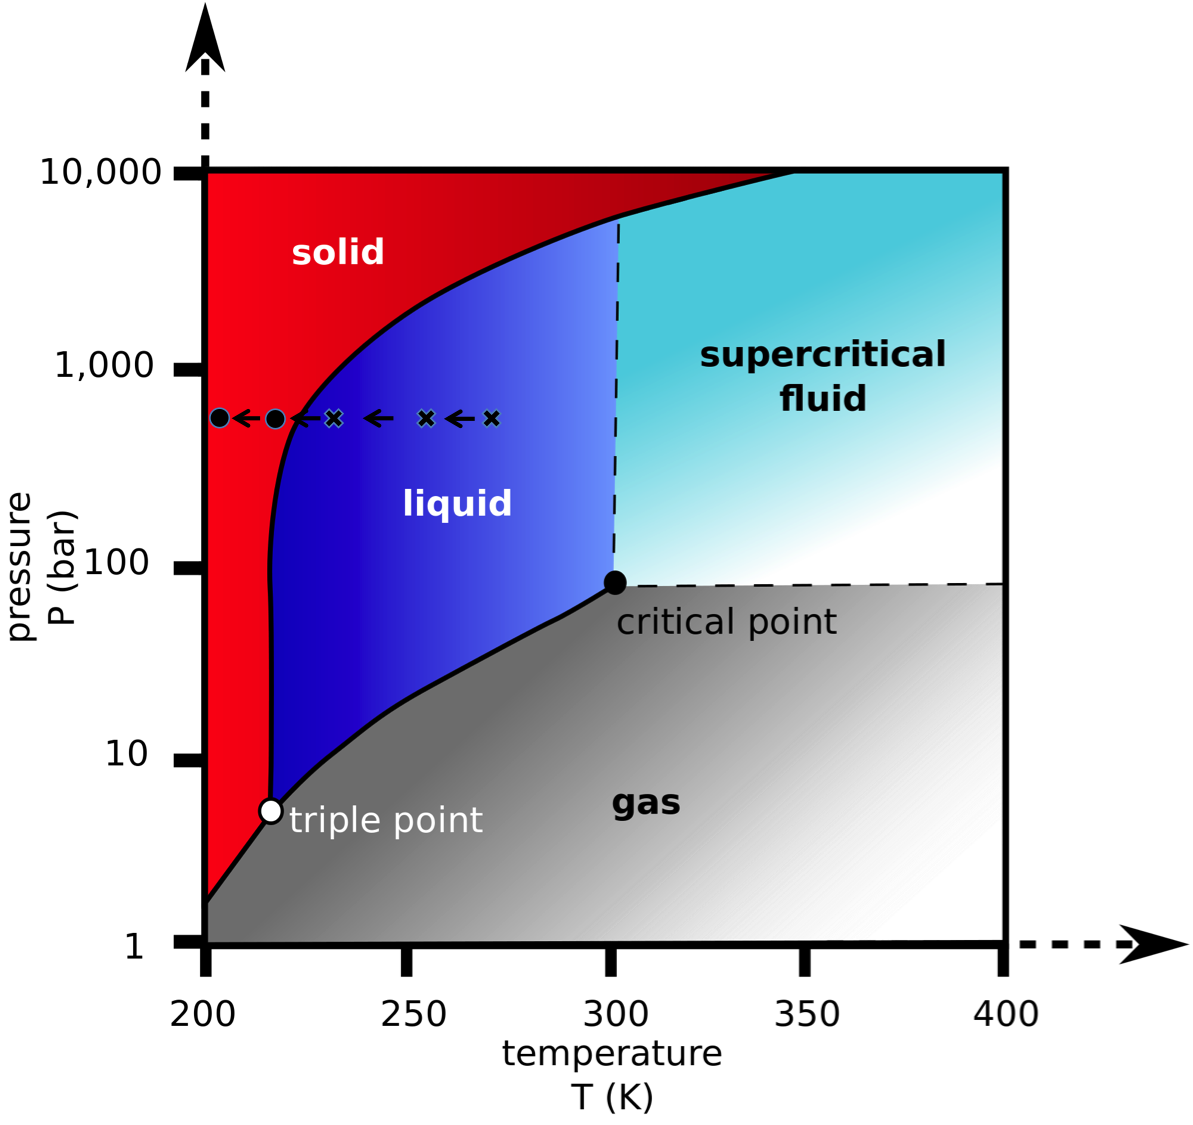
\includegraphics[width = .5\textwidth]{./Figures/Introduction/phase_diagram.png}
	\caption[An example of a schematic phase diagram.  There are phase regions, solid, liquid, gas, and a region known as supercritical fluid (liquid and gas become indistinguishable), each with a corresponding phase boundary dividing them.  A black x represents a system in a stable phase, and a black o represents a system in a metastable phase.]{An example of a schematic phase diagram.  There are phase regions, solid, liquid, gas, and a region known as supercritical fluid (liquid and gas become indistinguishable), each with a corresponding phase boundary dividing them.  A black x represents a system in a stable phase, and a black o represents a system in a metastable phase.\cite{EGELSTAFF}}
	\label{phase diagram}
\end{figure}

From Figure \ref{phase diagram}, the stable phase of a substance can be determined based on the substance's temperature and pressure.  The different phases are divided by coexistence lines, which indicate a state point in which both phases can simultaneously exist.  When the thermodynamic properties of a substance crosses a coexistence line, a phase transition may occur, in which the substance's physical properties change from one phase to another \cite{askeland2011the}.  Across these lines, there is a discontinuous change in physical properties such as density or entropy \cite{EGELSTAFF}.  However, this transition between phases can also be suppressed giving rise to the existence of supercooled or superheated phases \cite{askeland2011the}.  For example, a liquid substance cooled passed the coexistence line can exists as a metastable, supercooled liquid for various lengths of time.  This phase is considered metastable because the solid phase is knowingly more stable (the free energy of the metastable phase is greater than the stable phase).  However, there is a significant time for the substance to transition to the solid phase from the supercooled liquid phase \cite{Sear2016}.  This is shown in Figure \ref{phase diagram} by the black x's and o's.  The system begins as a stable liquid system, and is cooled beyond the coexistence line resulting in a supercooled liquid.

Once the coexistence line is reached or passed, the transition from one phase to another is initiated by the nucleation process.  Nucleation is the formation of a new phase or structure by re-organization within a preexisting phase or structure.  Nucleation can occur in two distinct manners.  First, known as heterogeneous nucleation, this is nucleation occurring along a container surface, an impurity, or a defect in the system \cite{Schmelzer2005}.  For example, heterogeneous nucleation occurs in the condensation along a water bottle edge.  The second form of nucleation is homogeneous nucleation, or nucleation that occurs in the bulk of a system, in the absence of impurities or surfaces \cite{Schmelzer2005}.  Heterogeneous nucleation occurs preferentially to its homogeneous counterpart, because the surface or impurity provide a seed to start the nucleation process \cite{Schmelzer2005}.  Nucleation results in a seed of the new phase.  This new phase, because it is energetically more stable, grows throughout the system until the new phase is ubiquitous in the system \cite{Schmelzer2005}.  As a result, there are two key rates in the formation of the new phase from a supercooled liquid phase, the nucleation rate and the growth rate, which are displayed in Figure \ref{overall_rates} \cite{barrett1973the}.

\begin{figure}[h]
	\centering
	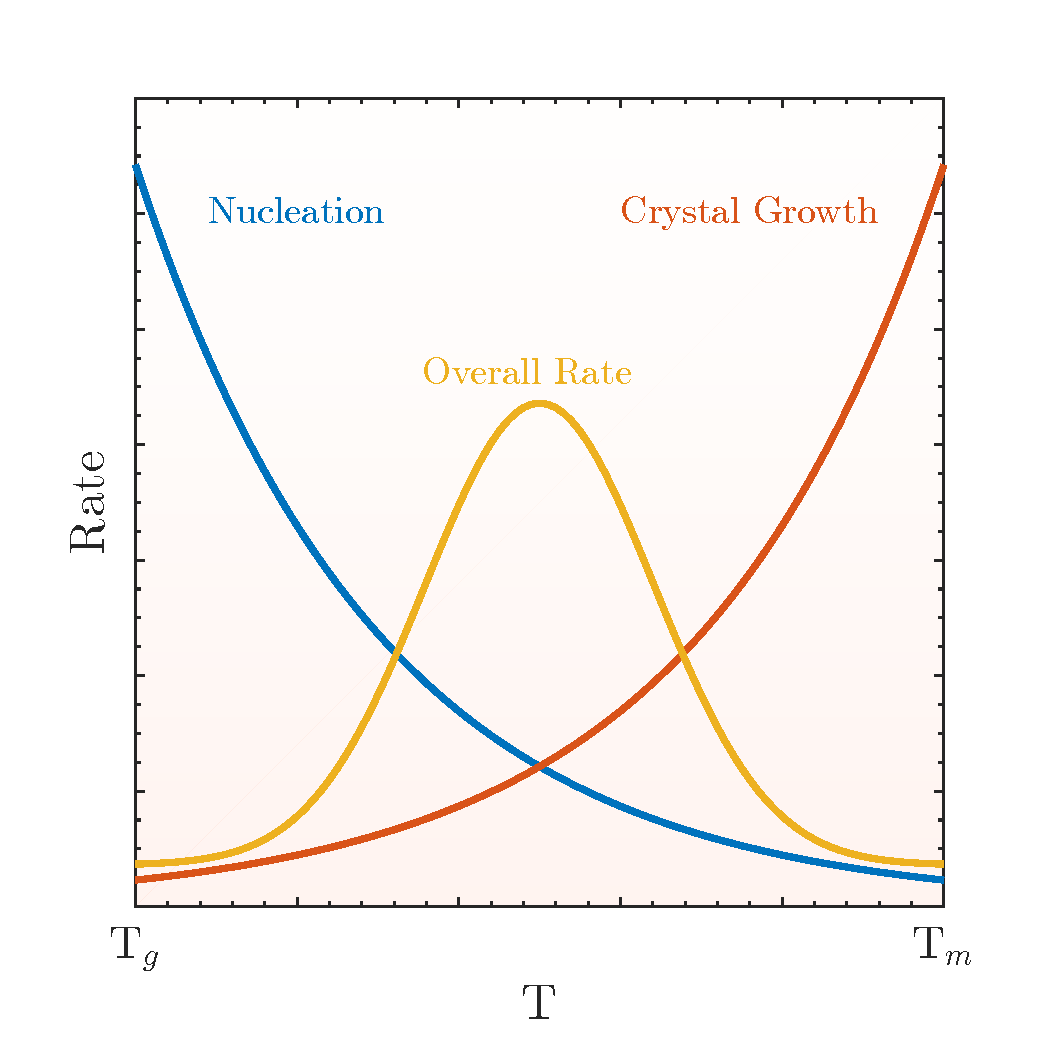
\includegraphics[width = .5\textwidth]{./Figures/Introduction/overall_rates.pdf}
	\caption[The theoretical nucleation, crystal growth rate, and the overall crystallization rate plotted versus temperature between the melting temperature, $T_m$, and the glass transition temperature, $T_g$.  The figure shows that crystal growth rates are larger at low subcooling because diffusion rates are higher at higher temperatures.  Similarly, the nucleation rate is higher at greater subcooling.  We assume that the overall rate for crystallization is the product of the two rates.]{The theoretical nucleation, crystal growth rate, and the overall crystallization rate plotted versus temperature between the melting temperature, $T_m$, and the glass transition temperature, $T_g$.  The figure shows that crystal growth rates are larger at low subcooling because diffusion rates are higher at higher temperatures.  Similarly, the nucleation rate is higher at greater subcooling.  We assume that the overall rate for crystallization is the product of the two rates. \cite{barrett1973the}\cite{Cavagna2009}}
	\label{overall_rates}
\end{figure}

Figure \ref{overall_rates} shows the two rates involved in crystal formation in a supercooled liquid, the nucleation rate and the crystal growth rate \cite{barrett1973the}.  The figure also shows the overall crystallization rate, which is the product of the nucleation and crystal growth rates.  The crystal growth and nucleation rates are shown to be monotonic as a function of temperature.  The crystal growth rate is low at high subcoolings because at low temperatures near the glass transition temperature, the dynamics of atoms is extremely slow.  As a result, atoms rarely move enough to combine with the nucleation site.  As the temperature is increased, the growth rate increases as the diffusion rate increases.  Conversely, the nucleation rate is low at low subcoolings, because fast diffusion rate leads to nucleation sites to dissipate before growth can begin.  As the temperature decreases, the nucleation rate increases because time for a nucleation site to dissipate decreases as dynamics slow.  Thus, the crystal growth rate has a maximum at the melting temperature, and the nucleation rate has a maximum at the glass temperature.  The overall crystallization rate is considered to be the product of the nucleation rate and crystal growth rate.  The overall crystallization rate has a maximum at an intermediate temperature between the melting temperature and glass transition temperature.  These results are shown in Figure \ref{overall_rates}.   The key feature predicted by theory is that different rates dominate in different temperature regimes, and the overall rate is non-monotonic.  Despite great effort devoted to the topic of nucleation, a complete understanding of the nucleation process from an experimental or computational approach is still lacking due to great difficulty in capturing the entire process.  

Experiments and simulations alike are very difficult to perform on the topic of nucleation, because nucleation is stochastic, transient, and atomic scale \cite{ReintenWolde1996}.  While experimental probes to capture atomic scale events exists, multiple nucleation sites often develop during experiments, and the deconvolution of the multiple nucleation events is difficult \cite{ReintenWolde1996}.  Similarly, traditional computational techniques such as molecular dynamics are limited in the timescales accessible.  Molecular dynamics is limited to the microsecond timescale, and the average time for a nucleation event to occur in a molecular dynamics simulation is beyond seconds.  It is the goal of this thesis to elucidate the true nature of the crystal growth rate and nucleation rate via metadynamics simulations.

Despite efforts to study nucleation experimentally, computationally, and theoretically, a complete understanding of the nucleation process of any phase transition is still incomplete \cite{Sanz2013}.  Understanding nucleation is an essential component to fully understand phase behavior in substances \cite{Reguera2013}.  The nucleation process influences the final crystal structure of substances with multiple polymorphs in the crystal phase \cite{Reguera2013}.  For example, nucleation can elucidate the origin of water freezing to one of seventeen different polymorphs at different state points \cite{Sanz2013}.  On the other hand, understanding the nucleation process can also provide new insight to the glass formation process.  Particularly, a complete understanding of nucleation may provide information about the origin of strong versus fragile glass formers, or the origin of good glass formers versus poor glass formers.  Nucleation also determines a material's transition from one crystal structure to another, which is of importance in electrical engineering.  Thus, an understanding of nucleation can provide insight on how to better predict and control the creation of materials.  Because the understanding of nucleation is essential to many fields of science and engineering, many nucleation theories have been proposed, the prevalent theory being classical nucleation theory.

Nucleation is traditionally described by classical nucleation theory (CNT) \cite{Sear2016}.  Classical nucleation theory assumes nucleation occurs via random density fluctuations resulting in nucleation sites of various size \cite{Sear2016}.  These sites will either collapse on itself or grow throughout the system depending on the size of the site.  The formation rate of these sites is estimated by the free energy barrier preventing the creation of these sites.  Classical nucleation estimates this free energy barrier with macroscopic quantities of the system.  Classical nucleation has been used alongside MD simulations \cite{Chkonia2009}.  CNT and MD has shown some success, but CNT is limited in its accuracy.  Many believe the short comings of CNT results from the approximations made to calculate the free energy barrier \cite{Chkonia2009}.  As a result, the goal of this thesis is to use metadynamics simulations to better estimate the free energy barrier involved in the nucleation process.

The remainder of this thesis will discuss our recent results on the homogeneous nucleation and crystal growth using metadynamics simulations to directly sample the energy landscape.  In chapter 2, we discuss classical nucleation theory, the prevailing method of explaining nucleation for decades, and discuss some of the pitfalls of the method.  In chapter 3, we discuss the metadynamics method used to directly sample the energy landscape as nucleation and crystal growth occur.  In chapter 4, the results of the metadynamics simulation are discussed.  In chapter 5, we discuss relevant differences between good crystal formers and good glass formers as shown by the energy landscape.  Lastly, in chapter 6, we summarize relevant conclusions and possible future work.  In the appendix section, honorable mentions are made to projects that support this research.